\required{Project Description}
\setcounter{section}{0}
\section{Introduction}
As sciences move towards more data driven research, data analysis has
become a main building block in a wide array of research disciplines.
Many advances in recent research have been driven by algorithmic improvements
in data analysis, in particular in predictive analytics and machine learning.
As machine learning becomes a tool for scientists across disciplines, it is
important that the neccessary analytical tools are freely available, and easy to use for
domain scientists outside of the field of machine learning.

% FIXME fast prototyping

The \sklearn{} machine learning library~\autocite{pedregosa2011scikit},
provides machine learning functionality within the established---and
growing---scientific Python ecosystem~\autocite{benlorica, infoworld}.
The \sklearn{} project is an open source project written in Python, implementing
state-of-the-art machine
learning algorithm and utilities to apply these algorithms to real-world data
analysis and prediction problems.
%
The distinguishing features of \sklearn{} are its generic and intuitive
interface, its comprehensiveness and its
documentation~\autocite{Varoquaux_2015, benlorica}.

\emph{\textbf{Interface}} \sklearn{} provides a generic interface for machine
learning, mainly consisting of only three methods: \texttt{fit}, to build
models, \texttt{predict}, to make predictions using models, and
\texttt{transform}, to change the representation of the input
data~\autocite{buitinck2013api}.
Table~\ref{api} illustrates this interface. The
simple and consistent interface helps to abstract away the algorithm, and let
users focus on their particular problem. The \sklearn{} project{} makes use of the
well-established NumPy library to represent data and predictions, minimizing
the friction of applying machine learning within an existing project.

\emph{\textbf{Comprehensiveness}} \sklearn{} implements a wide variety of
models for classification, regression, clustering and dimensionality reduction,
as well as methods for feature selection and feature extraction. The library
contains most of the algorithms included in standard textbooks like
\textcite{bishop2001bishop} and \textcite{friedman2001elements}, while
providing competitive implementation of state-of-the-art algorithms like
Gradient Boosting~\autocite{friedman2001greedy}, Random
Forests~\autocite{breiman2001random} and SAG~\autocite{roux2012stochastic}.  In
addition to a large selection of algorithms, \sklearn{} also contains a suite
of evaluation metrics and tools for parameter selection.

\emph{\textbf{Documentation}}
Documentation is a key ingredient to usability, and the documentation of \sklearn{}
has been widely recognized as an excellent learning
resource~\autocite{testimonials, benlorica, kdnuggetstopten, lovesklearn}. The
\sklearn{} project has strict rules on documentation and requires examples and
extensive descriptions for all algorithms.

The simple API together with the wide variety of algorithms that are
implemented in \sklearn{}, the package allows for very fast prototyping of
machine learning applications.
These key features are the ingredients leading to the wide-spread use of
\sklearn{}, and the creation of a large ecosystem of users, contributors,
maintainers and dependent packages.

\begin{table}
    \caption{Main \sklearn interface. All models have a \texttt{fit} method
    with the training data as parameter. Supervised models are also provided
    with the training targets or labels. New (usually multivariate)
    representations of the input data are produced by the \texttt{transform}
    method, while prediction of target variables (usually discrete labels or
    single continuous variables) or cluster memberships are produced with the
    \texttt{predict} method.
}
\begin{center}
    \begin{tabular}{p{.3\textwidth} p{.3\textwidth}}
    \multicolumn{2}{c}{\texttt{fit(features\_train, [labels\_train])}}\\\\
    \texttt{predict(features\_test)} & \texttt{transform(features\_test)}\\
    \cmidrule[1pt](r{1em}){1-1} \cmidrule[1pt](l){2-2}
    Classification & Preprocessing\\
    Regression & Dimensionality Reduction\\
    Clustering & Feature Selection\\
               & Feature extraction\\
    \end{tabular}
\end{center}
\label{api}
\end{table}

\section{Previous Impact of the \sklearn{} Package}
The \sklearn{} project has been widely used in academic and industrial research,
and has made its way into multiple commercial products. The
paper~\autocite{pedregosa2011scikit} describing \sklearn{} has been cited over 5.000 times
according to Google scholar\footnote{With nearly half of these citations
within the last year, showing accelerating growth.}.
Applications of \sklearn{} spread a multitude of research areas, including
Physics~\autocite{Baldi:2016fql, Yang:2016nnd},
Astronomy~\autocite{pereira2013spectrophotometric, bennett20141},
Biology~\autocite{misof2014phylogenomics, ritchie2014functional},
Medicine~\autocite{kamalov2015improving, ng2015computer},
Psychology~\autocite{park2015automatic,doehrmann2013predicting}, Cyber
Security~\autocite{sahs2012machine},
Oceanograpy~\autocite{sunagawa2015structure}, Social
Sciences~\autocite{driscoll2015searching, croicu2015improving} and more.

Other ways to measure the use and impact of \sklearn{} is the engagement with
the project via code contributions, downloads, support requests and other
community interactions.
According to the email addresses used for code contributions (a conservative
estimate), 40 researchers and students from at least 23 US universities
\emph{contributed code} to \sklearn{}, indicating wide-spread academic use.
These institutes include University of California Berkeley, Brown University,
Carnegie Mellon University, Columbia University, Duke University, Harvard
University, Massachusetts Institute of Technology, New York University,
Stanford University, and University of Washington.
The total number of unique contributors to the project is about 700.
%
The \sklearn{} mailing list has 1.666 subscribers, including 70 email
addresses from ``edu'' domains, across 43 institutes.
%
On the question-answering site Stack Overflow, there are around 7.000 questions
tagged as related to \sklearn{}.

The \sklearn{} project has become the center of the machine learning ecosystem
in the scientific Python community, with several domain-specific packages
relying on and extending its functionality.
Prominent examples of scientific software packages depending on \sklearn{}
for machine learning include \texttt{astroML}~\autocite{van2013openml} for astronomical
data, \texttt{nilearn}~\autocite{abraham2014machine} for neuroimaging, \texttt{MNE-Python} for MEG
and EEG data, \texttt{librosa}~\autocite{mcfee2015librosa} for audio and musical data,
\texttt{nltk}~\autocite{bird2006nltk} and \texttt{rosetta} for Natural language processing, \texttt{bcbio} for
RNA sequence analysis, \texttt{scikit-allel} for genetic variation data, and \texttt{rootpy} for
integration with the \texttt{ROOT} scientific software framework.
The main use of \sklearn{} is outside of these major open source packages, though,
as standalone library for data analysis. Using the GitHub repository, we found
about 120.000 Jupyter notebooks---a format for interactive computing with
Python---that use \sklearn{} at the time of writing\footnote{Up from 40.000 a year ago.}.

The \sklearn{} website containing the documentation was visited by over
930.000 users in February 2017, nearly doubling within the last year.

In addition to being widely used as a toolkit by practitioners,
\sklearn{} is also popular in teaching machine learning.
The emphasis on accessibility, usability and documentation within
the \sklearn{} project makes it ideal for an introductory
course in machine learning, and allows access to a wide variety
of algorithms.
Academic teaching has made use of \sklearn{} at institutes including New York
University, Brown University, Duke University, University of California
Berkeley, Stanford University, Princeton University, Columbia University,
University of Pennsylvania, Georgetown University, Cornell University and
others.

There have been several books have written about the use of
\sklearn{} including ``Introduction to machine learning with Python'' by PI
M\"uller.~\autocite{garreta2013learning, hackeling2014mastering,
hauck2014scikit, raschka2015python} 

\section{Proposed Work}
Despite the extensive documentation, applying machine learning using \sklearn{}
still requires expert knowledge about:
\begin{itemize}
    \item What kind of models to use for a given task.
    \item What kind of feature extraction and preprocessing is required for a model.
    \item What parameters to tune, and in which ranges.
\end{itemize}

While it is easy for a scientist to create a working model, this model might not
be optimum, and they could obtain a much better model using more expert knowledge
in machine learning to answer the questions listed above.
However, the need for this expert knowledge can be eliminated at least partially
using recent developments in model selection and
meta-learning~\autocite{NIPS2011_4443, feurer-nips2015,
snoek2015scalable, NIPS2012_4522}. While there exist attempts at
open source implementation for automatic model and parameter
selection~\autocite{bergstra2013hyperopt, komer2014hyperopt,
NIPS2012_4522, hutter2011sequential} and
meta-learning~\autocite{feurer-nips2015}, these implementations are
in the form of research prototypes that lack in terms of usability,
documentation, testing and integration into the existing
ecosystem.

Funding from this proposal would enable a concentrated effort to include more
automatic model selection in \sklearn{}, and therefore lower the barrier to
entry for applying machine learning even further.
The components of the proposed work are:
\begin{itemize}
    \item Improving the existing pipelining facilities for more automatic feature extraction.
    \item Recommend explicit sets of parameters to tune for each algorithm,
        together with recommended ranges, based on large-scale experiments.
    \item Integrate methods for Bayesian optimization for parameter selection.
    \item Integrate meta-learning for automatic model selection.
\end{itemize}
Together, these additions to the \sklearn{} ecosystem will enable more widespread use,
in particular by scientists outside of the field of machine learning, and improve results
of existing users.
Our goal is to improve the existing infrastructure for model selection in
\sklearn{}, and develop more novel features like meta-learning outside of the main
\sklearn{} package, for possible later inclusion.
To accomplish these goals, we will collaborate with the group of \emph{Prof.
Frank Hutter}, who are leaders in the current research on meta-learning, and
will allow us to built on their expertise.  We will also collaborate with the
group of \emph{Prof. Joaquin Candela} developing the OpenML platform, to make
sure their platform will support the needs for large-scale model comparison,
and will be able to provide easy access to our results.
We also established collaboration with scientists in multiple fields who apply
machine learning in their research, to ensure that the solutions we create are
applicable to a wide spectrum of domains.  These collaborations include
\emph{Prof. David Hogg} (Astrophysics and Astronomy), \emph{Prof. Kyle Cranmer}
(Experimental Particle Physics), \emph{Prof. David Sontag} (Medical Data
Analysis), and Prof. Chris Fonnesbeck (Biostatistics), as described in the
letters of collaboration accompanying this proposal. Their groups will adopt
the tools created in this project to provide early feedback on their usefulness
and provide use-cases to guide development.

\section{Intellectual Merit}
Improving automation in model selection and preprocessing in \sklearn{} will have far-reaching
implications for existing and future applications of machine learning.
Research projects that already use \sklearn{} for machine learning will be able to adapt better
models with minimal changes to their workflow, potentially improving their research outcomes.
For research projects that are not relying on machine learning yet, including a model
from \sklearn{} will be easier and require less expert knowledge.

Developing more automated model selection requires extensive benchmarking,
analysis and evaluation on a diverse array of machine learning problems. Such a
large scale evaluation, in the spirit of \textcite{caruana2008empirical,
caruana2006empirical} and more recently \textcite{feurer-nips2015} can provide
important insights into the state-of-the-art in machine learning. This proposal
will not only provide results of extensive evaluation, it will also result in
improved infrastructure for large scale studies of algorithms.
To evaluate the importance of the improvements, we conducted a community survey
among \sklearn{} users, which found a large demand for this functionality.
Details can be found in Section~\ref{community}.

\begin{figure}
    \begin{minted}[fontsize=\footnotesize]{python}
    # model fitting and prediction with fixed parameters:
    from sklearn.ensembled import RandomForestClassifier
    forest  = RandomForestClassifier(max_depth=10, max_features=3)
    forest.fit(features_train, labels_train)
    forest.predict(features_test)

    # model fitting and prediction with grid-searched parameters
    from sklearn.model_selection import GridSearchCV
    parameter_grid = {'max_depth': [1, 3, 10], 'max_features': [1, 2, 3]}
    forest_grid = GridSearchCV(RandomForestClassifier(), parameter_grid)
    forest_grid.fit(features_train, labels_train)
    forest_grid.predict(features_test)

    # grid-search with pipeline of feature selection, pca and random forest
    from sklearn.pipeline import Pipeline
    pipeline = pipeline([('select', SelectPercentile()), ('pca', PCA()),
                         ('rf', RandomForestClassifier())])
    parameter_grid = {'select__percentile': [10, 50, 90],
                      'rf__max_depth': [1, 3, 10], 'rf__max_features': [1, 2, 3]}
    grid = GridSearchCV(pipeline, parameter_grid)
    ... 
    \end{minted}
    \vspace{-5mm}
    \label{gridsearch}
    \caption{Current interface to \sklearn{} classification and parameter
        selection. The user needs to select parameters of importance (here
        \texttt{max\_depth} and \texttt{max\_features}), and values for these
        parameters to test (here 1, 3, 10 for \texttt{max\_depth} and 1, 2, 3
        for \texttt{max\_features}). Building more complex pipelines comprising
        multiple steps of feature processing complicates the process.}
\end{figure}

\section{Related Projects}
In this sections we briefly review related projects for machine learning in general
and more specifically automatic machine learning.

\subsection{Other Machine Learning Packages}\label{otherpackages}
The software tools used in the data science community can to a large degree be
separated by language, with Python and R by far the most popular choices, in
particular in research environments. Other languages include Java, Scala, C++, Lua and Julia.

While the R language has a rich ecosystem of tools for data analysis,
statistical modeling and machine learning, it has two major shortcomings:
Firstly, it is a domain specific language, specifically designed for statistic
applications. This makes it hard to integrate into existing software, or to
extend an R program to a web-service or a graphical user interface. Being a
special purpose language, there are few R programmers outside the field of data
analysis, making it harder to enter the field.
Python on the other hand is a general purpose programming language, and is being
widely adopted as the first programming language to be taught in schools and
universities, owing to its simple syntax and powerful libraries. Python is widely used
for user interfaces, web services and commercial systems.
Secondly, the software packages available for R are highly fragmented, without
common interfaces, often little documentation and lack of basic software development
practices like unit tests. Because Python is rooted in the programming community
rather than the statistics community, Python packages tend to have better software
development practices, including version control, documentation and testing. As point
of reference, the first unit testing framework in R was released in 2015, while a unit
testing framework is included in the Python standard libraries since 2001.

In Python, the most noteworthy related project is the relatively recent
tensor-flow. Tensor-flow is a framework for expressing computation graphs that
can be executed efficiently on many compute infrastructures from mobile phones to clusters.
Tensor-flow was designed for deep learning research, but can
be used more generically. Tensor-flow also
contains a module called tf.learn, which provides a high-level interface for deep learning,
mimicing the \sklearn{} interface.
Efforts on \sklearn{} and tf.learn are mostly orthogonal, with tf.learn
focusing solely on deep learning, with an emphasis on cutting edge research,
while \sklearn{} provides a wide array of time-tested methods for general
machine learning applications. Most improvements suggested in this project also
benefit the algorithms in tf.learn, as they focus on model-agnostic
infrastructure, and therefore can be used with the \sklearn{}
compatible tf.learn models.

Outside the Python and R languages, the two most widely used software tools are
the Weka environment writen in Java and machine learning software build on top
of the spark distributed computing framework (written in Scala).
Weka includes a graphical user interface (GUI), which is the primary way to interact with
the software.  Working within the GUI severely limits the available tools compared to
having the full flexibility of a programming language like Python or R.
Weka is meant for small-scale analysis and does not scale well to large datasets.

In contrast, spark is an abstraction build on a cluster computing
infrastructure and can scale elastically to datasets of nearly arbitrary size.
Spark includes the machine learning library MLLib, which contains a collection
of popular machine learning algorithms.
While Spark with MLLib is the only of all the tools we mentioned that is capable of
terrabyte-scale machine learning, only very few, highly specialize research projects have
enough data to justify the overhead of using a distributed solution. On smaller
datasets, solutions using a single machine are often faster, as they require less
communication and can implement a wider variety of algorithms~\autocite{rfbench}.

Weka and spark, as well as solutions in low-level, high-performance languages,
share a common problem for use in research: they are not designed for interactivity
with the user. There are no integrated ecosystems that would allow
interactive exploration of data, which is central to data-driven research.
For eaxmple, there are no mature scientific plotting libraries for either Java or Scala, so
generating something as simple as a bar chart or a confusion matrix can be
challenging.


\subsection{Existing Solutions for Automatic Machine Learning}
Within recent years, several implementations of automatic machine learning have
been published, usually as research software accompanying a paper. Many
available solutins are implementations of global optimization algorithms, such
as genetic programming and Bayesian optimization.
These packages provide a black-box optimization method, but require additional
work to define the search space and integrate with the actual machine learning
algorithms. Furthermore, these packages do not provide any meta-learning capabilities.
The hyperopt~\autocite{bergstra2013hyperopt} and
spearmint~\autocite{snoek2015scalable} packages are examples of this approach.
Both of these packages have been discontinued as their authors have left the academic
research community.
We are aware of four packages that attempt to solve the more integrated
end-to-end automatic machine learning problem:
auto-sklearn~\autocite{feurer-nips2015},
autoweka~\autocite{ThoHutHooLey13-AutoWEKA, kotthoff2016auto},
\texttt{tpot}~\autocite{Olson2016EvoBio, OlsonGECCO2016} and
\texttt{hyperopt-sklearn}~\autocite{komer2014hyperopt}. Out of these, only \texttt{auto-sklearn}
performs meta-learning.

As Auto-WEKA is implemented as a component of WEKA, it inherits its limitations
as outlined in Section~\ref{otherpackages}. 
The \texttt{hyperopt-sklearn} packages is a catalog of parameters for several \sklearn{}
models that allows automatic machine learning with \texttt{hyperopt} and
\sklearn{}. \texttt{hyperopt-sklearn} is not actively developed any more.
The \texttt{tpot} package uses genetic algorithms to build pipelines of
\sklearn{} models, but performs about as well as simpliy using a random forest
without parameter tuning~\autocite{OlsonGECCO2016}.
The \texttt{auto-sklearn} and related projects such as
\texttt{hyperband}~\autocite{li2016hyperband} represent the current
state-of-the-art in automatic machine learning, by performing automatic
parameter and model selection and meta-learning.
However, \texttt{auto-sklearn} has major restrictions that limit its usability,
such as no support for Windows or OS X, no support for the latest version of \sklearn{},
and a complex installation process. Furthermore, \texttt{auto-sklearn} does not provide
any feedback to the user before the whole search process is finished.
By coordinating efforts within \sklearn{} and \texttt{auto-sklearn} the proposed project
will improve upon these limitations, as well as extend the very basic meta-learning
algorithm implemented in \texttt{auto-sklearn}.



\section{Description of Activities}
%\enlargethispage{\baselineskip}
The goal of this proposal is to implement major usability and automation
features in \sklearn{}, decreasing the domain expertise required to
successfully implement machine learning models.  We propose to improve three
aspects of applying machine learning models that currently require substantial
expert knowledge: parameter selection, model selection and data preprocessing.

\subsection{Default Parameter Ranges}
Nearly all machine learning models come with hyper-parameters to set or tune
to achieve good predictive performance. The most wide-spread way to adjust
these parameters is grid-search with nested cross-validation.
Grid-search consists of an exhaustive search over all possible combinations
of the parameters under consideration. Example code for the process is given
in Figure~\ref{gridsearch}.
A major hurdle in applying grid-search in practice is that algorithms
often have many tuning parameters, making exhaustive search
over all of them infeasible. However, in practice only a small subset
of the parameters is usually critical for good performance. This set,
and good candidate values to try, are often not well-documented in research and
not included in text books.
The \sklearn{} documentation tries to give guidance, but can be hard
to find and understand by people outside of machine learning.
We propose the inclusion of a programmatic way to query for the parameters
to adjust for each model, and what good parameter ranges are.

While there is some community consensus on this issue, we want to back
up our choices by large scale experiments on existing benchmark libraries
of datasets, like OpenML~\autocite{van2013openml}. These enhancements will
be included directly in the \sklearn{} package.
\begin{labeling}{Task 1}
    \itemsep-4pt
    \item [Task 1] Analyze parameter ranges of commonly used supervised models.
    \item [Task 2] Provide default parameter ranges inside \sklearn{}.
\end{labeling}

\subsection{Bayesian Optimization Based Parameter Selection}
An alternative to exhaustive grid-search in selecting parameters is using
Bayesian optimization to iteratively improve the tuning parameters of a
model~\autocite{NIPS2011_4443, shahriari2016taking, NIPS2012_4522}. This
technique has been well-established in the machine learning literature, and
there are several implementations available.~\autocite{bergstra2013hyperopt,
feurer-nips2015, komer2014hyperopt, snoek2015scalable}.  However, these
algorithms have not made their way into the software used by domain scientists
that use machine learning algorithms as tools in their research.
By incorporating a robust and efficient implementation into \sklearn{},
this proposal will bring the benefits of the recent advantages in model selection
from the machine learning community to the scientific users of \sklearn{}.
\begin{labeling}{Task 3}
    \itemsep-4pt
    \item [Task 3] Analyze and integrate Gaussian Process based parameter optimization.
    \item [Task 4] Analyze Random Forest based parameter optimization.
    \item [Task 5] Integrate \texttt{auto-sklearn} Bayesian optimization with \sklearn{}.
\end{labeling}

\subsection{Automatic Preprocessing Selection}
The \sklearn{} package has a build-in mechanism to construct
``pipelines'' which are complex machine learning workflows, consisting of
operations like feature extraction, feature transformation, feature selection
and predictive models.  All evaluation and parameter selection mechanisms in
\sklearn{} can operate on these pipelines.
However, selecting which steps to chain together, that is which preprocessing
to use for which model, is left to the user. Currently there is no
automatic process to compare different pipeline constructions, even though
the right combination of methods is often crucial but not obvious in practice.
We propose to extend the model selection and pipelining framework in \sklearn{}
to allow automatic selection of pipeline steps.
%\enlargethispage{\baselineskip}
To help automatic preprocessing selection, we will also programatically
define input and output conditions of different processing steps, such
as requirements for sparse data, dense data, non-negativity of features and others.
\begin{labeling}{Task 9}
    \itemsep-4pt
    \item [Task 6] Allow setting of pipeline steps in \sklearn{} parameter searches.
    \item [Task 7] Implement tagging of pre-conditions and post-conditions for data transformations.
    \item [Task 8] Refactor \sklearn{} testing to validate pre-condition and post-condition tags.
    \item [Task 9] Collect common encoding schemes for categorical and
        continuous data in a \sklearn{} compatible way.
\end{labeling}

\begin{SCfigure}
    \centering
    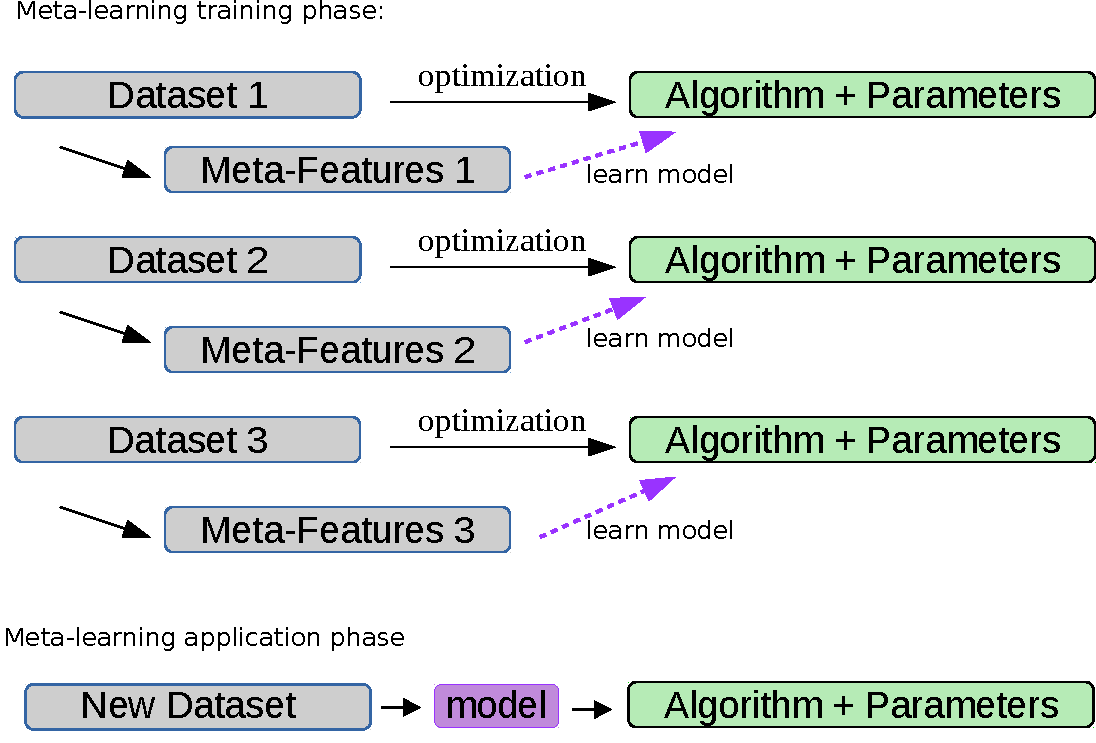
\includegraphics[width=.6\linewidth]{meta-learning-diagram.pdf}
    \caption{Illustration of meta-learning. First, good parameter values for
        each training dataset are found using optimization. Each dataset is
        then represented via meta-features. A Machine learning model is learned
        to predict parameter settings from the meta-features. For a new
        dataset, the machine learning model can be used to find good
    parameters, removing the costly optimization step.}
    \label{meta-learning}
\end{SCfigure}

\subsection{Meta-Learning}
Going beyond brute-force search or even Bayesian optimization for parameter and
model selection, it is possible to use machine learning to recommend suitable
algorithms and parameters based on properties of a data set, such as number of
samples, number of features, number of classes and statistical properties of
the features~\autocite{luo2015review, feurer-nips2015}.
Given these meta-features and the best pipeline and parameters found using
Bayesian optimization or grid-search, it is then possible to build a machine
learning model to predict what the best classifier for a new dataset would be.
This prediction based on meta-features is computationally much less demanding
than searching for a model and parameters from scratch for each new dataset.
Figure~\ref{meta-learning} illustrates the process.
Meta-learning allows the principled incorporation of expert knowledge as encoded
in the collection of datasets used for training.
While there are working implementations of meta-learning available
(\texttt{autoweka}, \texttt{auto-sklearn}),
these projects are currently in a ``research software'' state. Making these methods
available to the wider scientific audience will require substantial engineering
efforts. The previously described steps of incorporating Bayesian optimization
and automatic preprocessing selection will lay the foundation to enable
meta-learning within the \sklearn{} framework. These additions will likely not
be included in the main \sklearn{} package within the scope of this proposal,
but will be made available
as an additional package, compatible with and extending \sklearn{} functionality.
An illustration of the proposed additions is shown in Figure~\ref{additions_interface}.
\begin{labeling}{Task 10}
    \itemsep-4pt
    \item [Task 10] Refactor \texttt{auto-sklearn} to make use of new pipeline and transformation conditions.
    \item [Task 11] Analyze meta-learning features on OpenML datasets.
    \item [Task 12] Create meta-learning package from the previously build
        components, with full user documentation and test coverage that is
        installable via the Python package manager.
\end{labeling}

\begin{figure}
    \begin{minted}[fontsize=\footnotesize]{python}
    # model selection with default ranges
    from sklearn.model_selection import GridSearchCV, default_grid
    forest = RandomForestClassifier()
    forest_grid = GridSearchCV(RandomForestClassifier(), default_grid[forest])
    ... 
    # Bayesian optimization is an alternative to grid-search:
    from sklearn.model_selection import BayesianSearchCV
    BayesianSearchCV(RandomForestClassifier())
    ... 
    # allowing searches over pipeline steps
    from sklearn.model_selection import AutoPipeline
    pipe = AutoPipeline(RandomForestClassifier())
    BayesianSearchCV(pipe)
    ... 
    # meta-learning removes need to specify model or ranges:
    from metalearning import AutoClassifier
    classifier = AutoClassifier()
    classifier.fit(features_train, labels_train)
    ... 
    \end{minted}
    \vspace{-5mm}
    \label{additions_interface}
    \caption{Illustration of some of the proposed additions to the current
        \sklearn{} API\@. The \texttt{default\_grid} contains important parameters
        and ranges. \texttt{BayesianSearchCV} replaces the exhaustive search in
        \texttt{GridSearchCV} with Bayesian optimization. \texttt{AutoPipeline}
        searches over preprocessing steps, removes the need for users to
        specify them explicitly. Finally, \texttt{AutoClassifier} takes care of
        preprocessing and model selection via meta-learning.}
\end{figure}

\section{Enabled Research Opportunities}
The proposed project will benefit researchers inside the machine learning field,
but more importantly will have an impact on new and existing applications of machine
learning across many domains of science.

\subsection{Reduce Barrier to Entry}
One of the premier goals of this project is to lower the barrier to entry
to applying machine learning in scientific applications even further.
The \sklearn{} package with its intuitive interface and comprehensive documentation
has made machine learning algorithms available to a much wider audience.
However, selecting and tuning models still requires machine learning expertise.
The wealth of algorithmic choices for solving a particular research problem can be
overwhelming to researchers from other disciplines. By building more automated
abstractions on top of the existing machine learning algorithms in \sklearn{},
we will enable researchers to apply powerful models without learning
the characteristics and particularities of specific methods.
This will ease the adaption of machine learning for many researchers
that have not yet made use of machine learning.

\subsection{Improved Rapid Prototyping}
In data science, exploration is often limited by the human interactions needed to analyze data.
Being able to rapidly ask many research questions about a dataset or task of interest allows
quick exploration of hypotheses and speeds up research.
Data preprocessing and model tuning is often a laborious and time-consuming part of analysis.
More automation in applying machine learning means that a researcher can ask a scientific
question in terms of a machine learning problem, start the automated machinery to
search for a model, and then continue exploring the data, without having to closely monitor
the process on the model. 
This frees up research time to investigate other questions, instead of trying to
find the right model to answer the first.

\subsection{Plug-In Replacements}
Many researchers are already using \sklearn{} models in their projects, as witnessed
by the citations and other usage statistics we reported above. As the automation features
in this project will provide the same interface as the existing models, researchers
can replace the models in their existing projects by an automatic model search.
This will lead to better predictive results by only changing two lines of code.

\subsection{Large-Scale Comparisons}
Lastly, by providing a reproducible and open large-scale comparison of machine learning
methods on a wide variety of datasets, we provide guidance for future research
in machine learning itself.
In the tradition of \textcite{caruana2006empirical} and
\textcite{caruana2008empirical}, we will identify strengths and weaknesses of
existing models, to allow dissemination by the wider machine learning
community. By using the OpenML platform for model evaluation, we are
not only facilitating reproducibility of results, as all parameters and results
are stored on the platform, we are also enriching the information available on OpenML
by populating the database with our results.

\section{Community Engagement, Outreach, and Sustainability}\label{community}
\subsection{Community Survey}
To evaluate the importance of the proposed additions to the \sklearn{} user community
and to identify other possible aread of improvement we conducted a self-selected
survey of the \sklearn{} community. Using the \sklearn{} mailing list and social
media, we collected 372 responses, including 184 responses from users involved
in academic research~\footnote{The complete results can be found at https://www.surveymonkey.com/results/SM-RHGZVZ73/}.
When asked how likely they would make use of automated machine learning functionality
if it became available, 88\% of respondents replied they are "likely" or "very likely"
to use automated hyper-parameter search and 72\% replied they are "likely" or "very likely"
to use automatic model selection. When asked to pick the top 5 out of 14 possible areas of improvement,
38\% ranked automatic parameter selection within the top five, behind "Working with out-of-memory datasets" (57\%),
"Better pandas integration" (43\%) and "Easier visualization of data and models" (47\%).

\subsection{Community Integration}
As co-maintainer and member of the core team of developers of \sklearn{}, PI
M\"uller is well integrated into the development process of \sklearn{}.
This will enable the direct incorporation of many of the proposed enhancements
into the \sklearn{} main package.
It will also provide a wide exposure of the proposed activities to the
\sklearn{} community. We expect contributions to the proposed
project from the open source community from day 1 of this project.
The close connection of PI M\"uller to the \sklearn{} user community will
also enable us to closely interact with users to ensure covering common use cases,
instead of creating software solutions in the vacuum.

\subsection{Software Quality and Testing}
The \sklearn{} project has a history of high standards on code quality, reviews and testing.
Each new contribution to \sklearn{} needs to be reviewed by at least two senior team members
in addition to the contributor. Often, many more reviews are performed. The
pull-requests (contributions) made to the project have on average 16 comments
made by developers and maintainers on improving code quality and algorithms.

The \sklearn{} package has an extensive testing suite, covering 94\% of lines of code in the project.
The test suite consists of unit tests, integration tests and algorithmic tests.
Automated testing is performed on all algorithms in \sklearn{} to ensure a common
interface and user experience.
All tests are run as continuous integration tests on Microsoft Windows and Linux, and using
multiple versions of Python as well as multiple versions of \texttt{NumPy} and \texttt{SciPy}, ensuring
compatibility with a wide array of end-user systems.

In adding to the \sklearn{} project, this proposal will leverage the existing infrastructure
and quality standards inside the \sklearn{} community, ensuring high quality, well-tested code.

\subsection{Documentation and Distribution}
Similar to the processes for reviews and testing, the proposed project will
also be able to take advantage of the well-tested documentation and distribution
infrastructure of \sklearn{}.
The \sklearn{} project has a history of increasingly high standards for
documentation, requiring a description of algorithms, use cases, important
parameters and theory, as well as compelling examples~\autocite{lovesklearn,
benlorica}. This culture of comprehensive and accessible documentation will
carry over to any additions made as part of this proposal.

\subsection{Sustainability Plan}
The \sklearn{} community has grown substantially over the years, and volunteer efforts
are by far the largest component of work contributed to the project.
When people do leave for personal reasons, often time commitments made as part
of more senior academic positions, the project has managed to smoothly integrate new
contributors into the core team. Due to substantial efforts to ease the barrier
of entry for contributors, the \sklearn{} team is able to attract new volunteer
core developers on a regular basis, and has successfully transitioned from one
``generation'' to the next multiple times. 

While there is an active community around \sklearn{}, it is very hard to make
major changes based on volunteer efforts alone. New models that are added have
often been the product of internships or the Google Summer of Code program.  We
therefore propose to hire a full-time developer as part of this proposal to
greatly accelerate the progress in terms of usability and automation. Once
the proposed features are included into the project, maintaining them will be
possible using the resources provided by the community. 
% FIXME this argument needs to be way better.

% GSOC somewhere? Broader impacts?
\subsection{Diversified Outreach}
As part of this proposal, we plan to hold an annual workshop or coding sprint
in the New York area to engage scientists, and introduce them to contributing
to open source. Experience has shown that many people are interested
in contributing to open source, but are often intimidated by the process.
By hosting an open and interactive workshop, we aim to broaden the base
of contributors to the \sklearn{} project.
Unfortunately open source projects often lack diversity in their core team,
and most core contributors of scientific Python packages being men.
We hope to improve the situation by partnering with local and national
organizations for women in machine learning and women in the Python community,
to engage more female developers.
We plan a weekend-long workshop, which will give a short introduction to
contributing to open source, followed by two days of hands-on contributions to
\sklearn{}.
From prior experience~\autocite{meetupsprintSF}, it is possible for new
contributors to make meaningful changes within one or two days, so that
attendants will go home with a contribution to the project. After pioneering
this model with \sklearn{}, our goal it to engage with other open source
projects with core developers local to New York (\texttt{pandas},
\texttt{matplotlib}) to increase the impact of the workshop.

\section{Project Coordination and Evaluation Plan}
\subsection{Project Coordination and Timeline}
PI M\"uller is a core developer and co-maintainer of \sklearn{} and deeply integrated
into the community around it. The PI will lead the execution of the project and the integration
into \sklearn{} and the \sklearn{} ecosystem.
The developer will implement the new features and review changes proposed by
the \sklearn{} community. The developer will also perform and analyze large-scale
benchmarking experiments to validate the effectiveness of the parameter
recommendations and the automation features.  The PI and developer will both
interact with the greater community via issue trackers, mailing lists and
chat rooms. The developer and PI will share working space to aid close
collaboration. Figure~\ref{timeline} illustrates the timeline of the project.
\begin{figure}
    \begin{ganttchart}[
    hgrid,
    x unit=0.26cm,
    y unit chart=.5cm,
    compress calendar,
    time slot format=isodate-yearmonth,
    bar/.append style={fill=blue!50},
    include title in canvas=false,
    bar top shift=0.2,
    bar height=.6,
    bar label node/.append style={align=left, text width=7cm},
    y unit title=.3cm
    ]{2017-10}{2020-09}
    \gantttitlecalendar[title/.style={draw=none, fill=none}]{year}\\
    \gantttitlecalendar[title/.append style={fill=black!10}, title label font=\tiny\color{black!10}]{year}\\
    \ganttbar{1 Analyze parameter ranges}{2017-10}{2018-04} \\
    \ganttbar{2 Provide default ranges}{2018-05}{2019-4} \\
    \ganttbar{3 GP-base BO}{2017-10}{2018-10} \\
    \ganttbar{4 RF-based BO}{2018-05}{2018-10} \\
    \ganttbar{5 Integrate with \texttt{auto-sklearn} BO}{2018-11}{2019-10} \\
    \ganttbar{6 Searching pipeline steps}{2017-10}{2018-04} \\
    \ganttbar{7 Transformation conditions}{2017-10}{2018-04} \\
    \ganttbar{8 Integrate conditions in \sklearn{}}{2018-05}{2018-10} \\
    \ganttbar{9 Feature encodings in \sklearn{}}{2018-11}{2019-10} \\
    \ganttbar{10 \sklearn{} $\leftrightarrow$ \texttt{auto-sklearn} sync}{2018-11}{2019-10} \\
    \ganttbar{11 Analyze meta-learning}{2018-05}{2019-04} \\
    \ganttbar{12 Meta-learning packaging}{2019-11}{2020-9}
    %\ganttlinkedbar{Task 2}{3}{7} \ganttnewline
    %\ganttbar{Final Task}{8}{12}
    \end{ganttchart}
    \vspace{-5mm}
    \caption{Project timeline}%
\label{timeline}
\end{figure}

\subsection{Need for a Senior Developer}
As many of the contributors of \sklearn{} work in academic environments,
often the time they have available to do volunteer work on open source is
inversely proportional to their seniority.
Consequently, there are many junior contributors with good coding skills,
but less developed project management and timing skills.
Therefore, it is paramount to have a senior developer to lead the efforts
on major new features, to ensure roadmap and scoping are useful and realistic.
The \sklearn{} project has around 430 open contributions (GitHub pull requests) at the moment,
which require code review and oversight from a senior developer to be integrated
into the project. This exemplifies the size of the community of contributors,
but also points out the bottleneck in terms of senior developers that
have enough machine learning and software development expertise to judge
the usefulness, efficiency and correctness of the proposed additions.


\subsection{Evaluation}
The success of an open source project is notoriously hard to measure. The
success and impact of an addition to an existing open source project even more
so. Open source software has many paths of distribution, few of which can
be tracked reliably.
The number of citations of the relevant paper~\autocite{pedregosa2011scikit}
could be used instead, but is likely to underestimate the number of research
projects using the \sklearn{} library in their research, as software is often
not cited.

To get a more comprehensive picture of the adoption of an open source software
we can look at other statistics like the number of discussions on the question
answering site Stack Overflow, the number of contributors, the number of people
writing to the mailing list, the number of projects depending on the package
etc. These numbers are particularly meaningful when compared to other projects
with a similar scope.

We will develop the more novel features outside of the \sklearn{} package, which will
ease measuring the impact of the proposed additions. For the components that will
be integrated into \sklearn{}, one simple measure of impact
is that it is actually be integrated into \sklearn{}.
Even though the PI is tied into the core developer team, there is no guarantee
a contribution will be accepted unless it meets the very high standars
on code quality, usability and usefulness set by the community.

Another direct measure of impact is to count use of a particular function in
code available on GitHub. As more and more research groups use version
control for their experimental code, and publish it as open source, a growing
number of groups and individual researchers have a presence on GitHub.com.
Counting the use of the added functionality, in particular inside Jupyter
Notebooks, provides great insight into the use of the proposed additions in
research and data analysis.

In addition to measuring the usage of the project outcome, we will also measure
the effect of using the implemented improvements on ease of use and efficiency
of implementing machine learning algorithms.
We will do so by conducting user studies with students at the Columbia University
Data Sciencie Institute. The study will measure time spend to arrive at a solution
for supervised machine learning problem, accuracy of the produced solution,
and a qualitative evaluation of user experience.


\section{Collaborations}
\subsection{Diversity in Open Source in Collaboration with WiMLDS}
While the \sklearn{} community is quite successful in finding new contributors,
unfortunately only one of the 38 \sklearn{} core developers is a woman.
Similar issues can be found in related packages, with \texttt{NumPy} having no
woman among the 13 core developers and \texttt{SciPy} having one woman out of
22 core developers.

To increase diversity, this proposal includes an annual workshop to increase
contributions to the open source community, in particular targeted at women.
To this end, we collaborate with the ``Women in Machine Learning and Data Science''
meetup group located in New York, a community of over 1.500 (mostly) female data science and
machine learning experts.

\subsection{Collaboration with \texttt{auto-sklearn}}
The \texttt{auto-sklearn} project~\autocite{feurer-nips2015} currently provides
a research prototype of meta-learning with Bayesian optimization for parameter
selection. One of the main goals of this proposal is to transfer the research
within the \texttt{auto-sklearn} project to an easy-to-use and well-documented
library, integrated within the \sklearn{} ecosystem. To this end, we will
collaborate with the \texttt{auto-sklearn} team, building upon their insights
and technologies. \emph{Prof. Frank Hutter} committed to providing the support of his group
to integrate our additions to \sklearn{}, such as the default parameter ranges
and automated preprocessing selection into their software, while in turn
providing the necessary domain knowledge to reproduce their research results in
a user-friendly library.

\subsection{Collaboration with OpenML}
Evaluation and benchmarking on real-world datasets are essential to this
proposal, in providing guidance for good parameter ranges, and assessing the
success of automatic model selection methods. The OpenML
project~\autocite{van2013openml} provides a quickly growing database of machine
learning datasets with associated tasks, including classification and
regression~\autocite{vanschoren2014openml}. Currently, there
were nearly 20.000 datasets hosted on OpenML, ranging from classical datasets
like MNIST and small toy datasets like the iris dataset, to large
scale datasets with millions or even tens of millions of samples, from domains
including as biology, medicine and physical sciences and commercial applications.
This growing collection of research datasets provides the basis of our
assessments, and ensure relevance of our effort across research domains.
\emph{Prof. Joaquin Candela} committed to improving and maintaining the Python
interface for the OpenML platform, and improving the support for \sklearn{}
based models.

\subsection{Early Adopters}
The following researchers have committed to being \emph{early adopters} of our
software products. They will use the improvements and packages in their
research projects, and provide valuable feedback for ensuring usefulness of the
software for a variety of research applications:

\paragraph{Experimental Particle Physics}
\emph{Prof. Kyle Cranmer} (NYU) committed to have his group be an early adopter of the
proposed project for their work on searching new phenomena at the Large Hardron
Collider.

\paragraph{Astronomy}
\emph{Prof. David Hogg} (NYU) committed to have his group be an
early adopter of the proposed project their projects in astronomy and
astrophysics. In particular, they will apply the developed methods in their
work to calibrate imaging spacecraft (like the GALEX and Kepler missions) and
in their data-driven models of stars (exemplified by our project called The
Cannon), as well as related projects.

\paragraph{Medical Data Analysis}
\emph{Prof. David Sontag} (NYU) commited to
have his group be an early adopter of the proposed project for their
work on building risk stratification algorithms for early detection of type 2 diabetes.
Building their models involves a significant amount of iteration over
approaches to regularization, the type of data to include in the model, and
different ways of deriving features from the data, which could potentially be
automated using the software described in this proposal.

\paragraph{Biostatistics}
\emph{Prof. Christopher Fonnesbeck} (Vanderbilt
University) committed to be an early adopter of the proposed project in
his work in statistical of biomedical data in epidemiological
applications, such as the control of infectious disease. This work
includes building of classification and regression models for
meta-analysis, with the goal if supporting evidence-based medicine.

\section{Broader Impacts}
The proposed project has a wide-reaching impact on the practical use of
machine learning in research, and on how machine learning can be taught to
 scientists from other domains.
Providing more automatic model selection will drastically lower the barrier
to entry to using machine learning for people without domain expertise
in machine learning.
Additionally, it will save time and effort spend by researchers doing
model selection by hand, replacing their effort by an automated process.
This will make researchers more productive, and will allow them to focus
on their area of study.

Automation, coupled with publishing the results of large scale experiments will
also provide help in education. Currently, often parameters and preprocessing
are seen as undocumented expert knowledge, derived from personal experience.
Formalizing this knowledge, and providing a database of experiments, will allow
students to quickly master the necessary steps to apply machine learning in
practice.

The proposed project will also enable us to grow the open source community
within the data science and machine learning community.  In particular, the
position of \sklearn{} as a popular and valued research library enables us to
reach out to a broad community of users.  The prominent status of \sklearn{}
enables us to influence the current make-up and values of the scientific open
source ecosystem.  We proposed to host ``coding sprints'' to introduce
outsiders to contributing to open source and enlarging the number of
contributors even further. This event will be held collaboration with the New
York based Women in Machine Learning and Data Science group, to grow the number
of female contributors in particular. 

% as in the project summary, broader impacts must be called out separately 
% in the project description.  You may be able to give more specific
% examples, or discuss how you've previously achieved these impacts.
% It should be similar, but not identical, to the Broader Impacts statement
% in the project summary

\section{Results From Prior NSF Support}
Dr.\ Andreas M\"uller has not been a PI or co-PI on an NSF grant.
